\documentclass[../main.tex]{subfiles}
\graphicspath{{\subfix{..}}}
\begin{document}
\chapter{Joint fit between the SPMT and LPMT spectra}
\epigraph{``We demand rigidly defined areas of doubt and uncertainty!''}{Douglas Adams, The Hitchhiker’s Guide to the Galaxy}
\label{sec:joint_fit}
% I)  Introduction globale.
% -------------------------------------
% ... Aborder les points suivants de manière succinte, pour donner une vision d'ensemble...
%
%     + JUNO est une expérience de physique de précision : il sera indispensable de comprendre très précisément les effets de reconstruction. C'est  d'autant  plus un défi que Juno emploie une technologie standard en physique des neutrinos (sphère ou cuve de scintillateur liquide  + PMT) mais l'amène dans une configuration extrême et inédite (très gros volume de scintillation, PMT de 30 pouces, etc...) où comprendre les effets de détection peut s'avérer difficile. Il est possible de rater quelque chose. Pouvoir comparer les données et résultats issus de deux systèmes indépendants, soumis à des problèmes différents, est donc précieux. C'est l'origine du dev de sPMT en plus des LPMT.
%
%     + L'importance cruciale de la maîtrise de la reconstruction : résolution à mieux que 3% et biais très inférieur à 1% sur la connaissance de la non linéarité sous peine d'incapacité à mesurer la NMO.
% Rappeler cet élément majeur : si on se trompe de 1%, on conclut à la mauvaise NMO. Utiliser la figure donnée dans la thèse de Yang pour appuyer ce point.
%
%    + Une source possible de non linéarité difficile à détecter à ce stade est la QNL. (Voir section suivante pour définition complète).
%
%     + La DC répond à cela. Elle interviendra notamment en fournissant des méthodes de calibration permettant de corriger la QNL. Ne pas en dire plus, ref these Yang.
%
%     + Plus generalement : Comparer deux systèmes pour détecter des problèmes sur la calibration ou la reco de l'un des deux. C'est ce que l'on fait dans cette thèse en comparant directement les résultats de la mesure des params d'oscillation.
%
%    + Une difficulté à étudier : la corrélation entre les deux systèmes : pas suffisant de comparer l'écart entre les valeurs centrales aux incertitudes individuelles. Nous proposons dans ce chapitre une exploration préliminaire testant différentes méthodes, en prédisant la sensibilité de ces méthodes à la présence QNL à divers degrés.
%
%   + Plan du chapitre.

JUNO is an experiment of precise measurements, where we try to observe small fluctuation in the energy spectrum and have the ambition to achieve sub-percent precision on the oscillation parameters measurement. It is crucial to understand extremely well the reconstruction and the effect we are dealing with. The challenge reside in the standard technology used in the detector, scintillator observed by PMT, but in a scale never seen before, for scintillator volume as for its PMT. Understanding every effect that goes in the detector can become extremely complicated. Being able to compare the results of the same experiment with two systems is thus precious, this is the origin the dual calorimetry with the LPMT and SPMT system.

The resolution and bias of the reconstruction needs to be extremely well characterized: the target resolution of 3\% \cite{juno_collaboration_juno_2022} is unprecedented as is required to be able to distinguished between Normal Ordering (NO) and Inverse Ordering (IO). The non-linearity uncertainty needs to be contained under 1\% or the risk appear to measure the wrong ordering \cite{han_dual_2021}.

One of the possible non-linearity source, that will be used as a reference source in this chapter, is the charge non-linearity (QNL) that will be detailed in next section. The dual calorimetry will be able to solve this problem, using calibrations method and measurements that will be used to correct it \cite{han_dual_2021}.

More generally, comparing the results of the two system will allow to detect potential issues on the calibration or reconstruction. This is done in this thesis by comparing directly the spectra and oscillation parameters measurements of the two system.

The study of the independents results of the two system can bring some informations \cite{cabrera_multi-calorimetry_2023} but this is missing the important correlation that should be present between the two system: they see the same events, in the same scintillator, their bound to be correlated. We explore in this chapter a preliminary study of the impact of those correlation via multiple methods and the impact of QNL at various degree.

In the next section will discuss the motivations behind this study. In section \ref{sec:joint_fit:approach}, I present the approaches and assumptions in this study. In section \ref{sec:joint_fit:framework} I present the fit framework used and following in section \ref{sec:joint_fit:tech} the technical improvement brought and the difficulties faced during the development. To end this chapter I present the results in \ref{sec:joint_fit:results} and discuss the conclusion and perspectives in \ref{sec:joint_fit:conclusion}.

\section{Motivations}
% II)  Motivations
% --------------------------
%
%   (a) Écart entre les résultats sPMT et LPMT
%       -- Tout écart significatif entre les résultats obtenus avec les deux systèmes signale un problème, et est donc intéressant, quelle que soit l'origine du problème.
%      -- Les deux systèmes ont une sensibilité équivalente à theta_12 et dm2_12. Ce sont donc ces deux paramètres que nous comparerons.
%     -- Pour détecter un écart significatif, on ne peut se contenter de comparer l'écart à la racine de la somme quad des erreurs individuelles. En effet, une grande partie de l'incertitude provient des incertitudes statistiques sur le spectre vrai de l'énergie des antineutrinos. Ce spectre étant le même pour les deux systèmes, les erreurs stats sur spectres reconstruits par les deux systèmes sont très corrélées. Si la reconstruction de l'E avait une résolution et un biais nul dans les deux systèmes, alors l'incertitude statistiques entre les mêmes bins des deux spectres serait 100% corrélée. Dans la réalité, les effets de reconstruction, en partie aléatoires, diminue cette corrélation. Elle reste néanmoins un élément central dans ce travail.
%
%    -- Notre travail dans cette partie de la thèse a été de mettre au point plusieurs tests statistiques pertinents pour détecter un écart entre le système des LPMT et celui des sPMT.
%      + Un premier objectif est de fournir les distributions des tests statistiques dans le cas où il n'existe pas de source de désaccord imprévue entre les deux systèmes. La valeur obtenue dans les données réelles pourra être comparée à ces distributions pour déduire des p-values.
%     + Pour évaluer une sensibilité, nous avons besoin de simuler une différence concrète. Nous choisissons de nous intéresser à un effet plausible, la QNL (voir prochaine sous-section). Nous soulignons cependant que la méthode peut être utile quelle que soit la source d'une différence entre LPMT et sPMT (problème dans la calibration, réglage fin de la simulation insuffisant pour un bon data/MC, etc...)
%
\subsection{Discrepancies between the SPMT and LPMT results}

As discussed in the introduction of this chapter, the SPMT system and the LPMT system will observe the same events. This mean that, after calibration, if the two system show significant differences in their results this is the signal of potential overlook of an effect or problem. Being able to detect such differences is thus crucial as, as discussed above, even the smallest deviation from our model could lead to the impossibility to measure the Mass Ordering (MO) or even worse, wrong our measurement.

The two system are expected to have the same sensitivity to the oscillation parameters $\theta_{12}$ and $\Delta m^2_{21}$ \cite{juno_collaboration_sub-percent_2022}. We will thus rely on the measurement of those two parameters to detect potential discrepancies.

We could just look at the value and compare them to the estimated independent error of the two system, but we believe and will demonstrate in this chapter that the independent study of the two system is missing a lot of informations, and that, by taking into account the statistic and systematic correlations between the two systems, we can produce much more powerful statistical test.

Our work in this chapter is to develop such tools. The first step is, of course, to verify that in the case of no discrepancies, the results are coherent with the independent analysis. This will give us the distribution of those statistical test in absence of discrepancies. When we will have real data, we will be able to compare it to those distribution to obtain a p-value characterizing the absence of those potential discrepancies.

To evaluate the power of our methods, we need to simulate a concrete discrepancy. We decide to study a plausible effect, the Charge Non-Linearity (QNL) that is detailed next section, but the goal of those tools is to be discrepancy agnostic, as those discrepancies could come from a variety of source (calibration issue, insufficient simulation tuning, etc...)

%
%   (b) Explications sur la QNL. (  ~ 1 p)
%
%       -- Rappeler que la réponse en E du détecteur est sujette à plusieurs sources de non linéarité. La principale est la NL dans la scintillation de photons. Une autre source est la QNL.
%
%      -- Définition, origine, etc.
%
%      -- Une façon de modéliser : la formule de Yang sur les Q_LPMT.
%          * Insérer les figures que tu as produites récemment (voir slack le 8 juillet à 17h39 et 17h52) : N_ph/N_ph_qnl vs. Etrue, pour différentes valeurs de gamma_qnl. Cela permet au lecteur de rapidement comprendre l'impact du PB.
%         * Fais le lien entre alpha_qnl et gamma_qnl, pour expliquer que plus tard, on ne testera que avec alpha_qnl, c'est à dire en simulant un effet global sur l'Erec pour générer plus vite.
%         * Dans ces figures, tu t'arrêtes à gamma_qnl = 1% <=> alpha_qnl = 0.3 %, je pense que tu peux aller jusqu'au 5% (regarde ce qui est fait chez Yang et dans la publi multicalo). Aussi bien à 0.5%, qu'à 1% et  qu'à 5%, donne le alpha_QNL correspondant, puis introduis-le dans IBDgen pour produire une spectre oscillé biaisé par la QNL, à comparer dans une figure au spectre sans QNL. Le but est de donner une idée de l'impact sur la NMO.
% En tout cas convaincre qu'il y en a un. Si Steven peut produire un delta-chi2, ce serait super.
%
% Remarques :
%       -- C'est un point important, donc il faut que cela soit auto-contenu au maximum.
%       -- S'inspirer de la publi multicalo, et de la thèse de Yang.
%       -- Citer ces deux sources, mais seulement en complément.
%

\subsection{Charge Non-Linearity (QNL)}
\label{sec:joint_fit:qnl}

The CD energy response is subject of two kind on non-linearity, the first one is the LS response non-linearity where the LS photo-production is not linear with the deposited energy as illustrated in figure \ref{fig:juno:nl:gamma}. The second one is the LPMT response non-linearity where the charge read from the LPMT is not linear in respect to the number of collected Photo-Electron (PE) (see section \ref{sec:juno:calib}).

The LS non-linearity comes from physics sources. Particles interaction in the LS will produce mainly scintillation light as discussed in section \ref{sec:juno:LS} but will also produce some cherenkov light (< 10\% of the collected light). Both mechanisms posses intrinsic non-linearity, for the Cherenkov emission it's dependent on the velocity of charged particle velocity while the scintillation photon-yield follow a so-called Birk's law with a "quenching" effect depending on the energy and type of particle \cite{particle_data_group_review_2020}. This results in a event-wise QNL.

The LPMT response non-linearity can come from sheer saturation when subject to a high rate of photon inducing a gain non-linearity or come from readout effects such as the electronic noise, the overshoot, the integration time window and even the waveform algorithm. All of those effects results in a channel-wise QNL.

Precedent studies \cite{han_dual_2021} suggest a model to emulate this non-linearity response that will be used in this work. We thus define the channel wise non-linearity that would be applied to each LPMT readout
\begin{equation}
  \label{eq:joint_fit:gamma_yang}
  \frac{Q_{rec}}{Q_{true}} = \frac{-\gamma_{qnl}}{9} Q_{true} + \frac{\gamma_{qnl} + 9}{9}
\end{equation}
where $Q_{rec}$ is the reconstructed number of PE by the PMT, $Q_{true}$ is true number of PE that hit the PMT, and $\gamma_{qnl}$ is a factor representing the amplitude of the non-linearity.

We also define an event-wise non-linearity characterized by
\begin{equation}
  \label{eq:joint_fit:alpha_yang}
  \frac{E_{vis}}{E_{true}} = \frac{-\alpha_{qnl}}{9} E_{true} + \frac{\alpha_{qnl} + 9}{9}
\end{equation}
where $E_{vis}$ is the visible energy that can be collected by the detector and $E_{true}$ is the true deposited energy. An example of the effect of such event-wise QNL is presented in figure \ref{fig:joint_fit:spectrums_comp}.

\begin{figure}[ht]
  \centering
  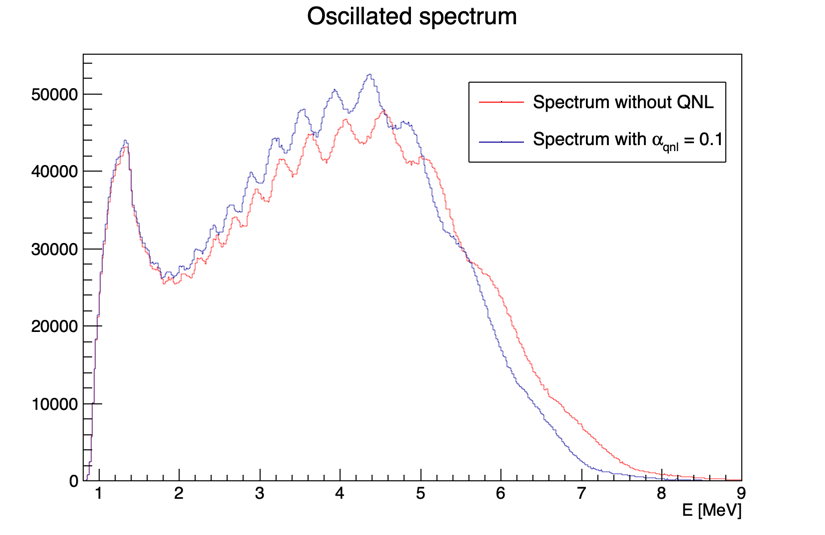
\includegraphics[height=5cm]{images/joint_fit/spectrums.png}
  \caption{Two oscillated spectrums of 1e7 event expected in JUNO. In red the spectrums without supplementary QNL. In blue the same spectrum but where an event-wise QNL $\alpha_{qnl} = 10\%$ is added.}
  \label{fig:joint_fit:spectrums_comp}
\end{figure}


Using 1M from the JUNO official simulation J23.0.1-rc8.dc1 (released the 7th January 2024), we simulated events up to the photon collection in LPMTs and simulated an additional channel-wise QNL by applying the equation \ref{eq:joint_fit:gamma_yang} to the number of collected photons.

\begin{figure}
  \centering
  \begin{subfigure}[t]{0.48\linewidth}
    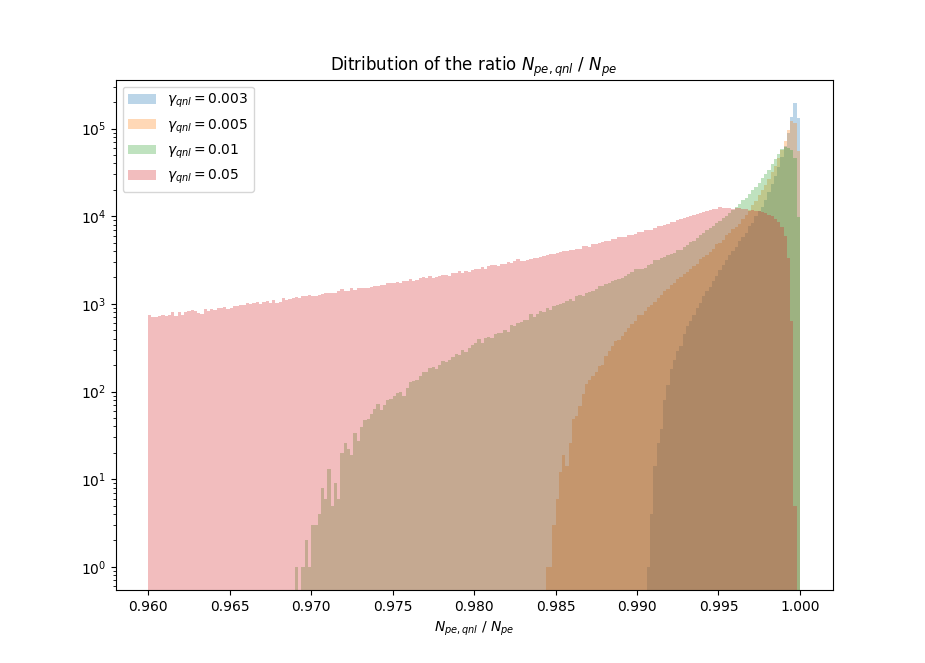
\includegraphics[width=\linewidth]{images/joint_fit/gamma_eff.png}
    \caption{Distribution of ratio of collected nPE after the additional QNL over the number of nPE that would be collected for different $\gamma_{qnl}$. We select event with an interaction radius $R < 4$m to not be affected by the non-uniformity.}
    \label{fig:joint_fit:ratio_distrib}
  \end{subfigure}
  \hfill
  \begin{subfigure}[t]{0.48\linewidth}
    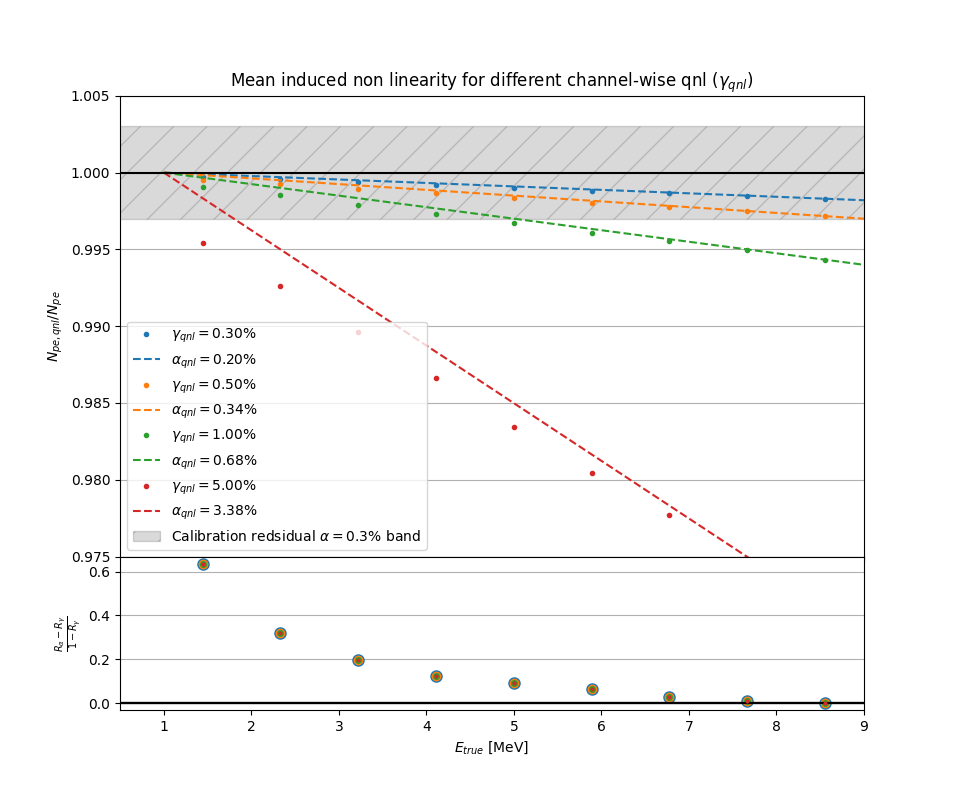
\includegraphics[width=\linewidth]{images/joint_fit/gamma_to_alpha.png}
    \caption{Ratio of collected nPE after the additional QNL over the number of nPE that would be collected at different energies. We select event with an interaction radius $R < 4$m to not be affected by the non-uniformity. The dots represent the mean of the distribution in figure \ref{fig:joint_fit:ratio_distrib} and the dashed line are the equivalent event-wise non-linearity from eq \ref{eq:joint_fit:alpha_yang}. The hatched zone is the residual non-linearity expected after calibration \cite{juno_collaboration_calibration_2021}.}
    \label{fig:joint_fit:gamma_v_alpha}
  \end{subfigure}
  \caption{}
\end{figure}

In figure \ref{fig:joint_fit:ratio_distrib} we show the the distribution of the ratio $\frac{Q_{rec}}{Q_{true}}$ for central events ($R < 4$m) and different value of $\gamma_{qnl}$. In figure \ref{fig:joint_fit:ratio_distrib} we show the mean of this distribution as function of the energy. We show effective $\alpha_{qnl}$ for each value of $\gamma_{qnl}$. We see that using the event-wise QNL is equivalent to the mean behavior of using channel-wise QNL.

When using channel-wise non-linearity, we need to simulate a number of PE per LPMT, the process can be quite tedious if we want a realistic simulation so in this study we are only using event-wize non-linearity to make the process simpler. This event-wise non-linearity will be characterized by $\alpha_{qnl}$.

%  (c) Blinding ?
%  L: Pas expert du sujet (mais alors pas du tout). Je me souviens de la discussion avec steven ou on pourrait ainsi appliquer nos outils avant l'unblidding et ainsi verifier que tout vas bien avant de regarder les resultats ?
%
%
%  (d) Motivations techniques
%
%       -- À compléter à partir de mes notes.
%          Tourne autour de la capacité, utile en général, à réaliser un fit joint.
%  L: En gros dire que c'est pratique de savoir le faire ?

\section{Approach}
\label{sec:joint_fit:approach}

In this section we detail the testing procedure behind each of our tools.

% III) Démarche
% -----------------------
%
%   (a) Simulation d'échantillons toys.
%
%          --- C'est la base de cette étude.
%          --- Dans chaque toy, nous générons un spectre vrai de l'E_nu qui est le point de départ commun de la production des deux spectres reconstruits des LPMT et des sPMt.
%          --- Puis nous ajoutons de façon simplifiée (pas nécessaire d'en dire plus ici, voir la sous - section sur IBDgen) les effets de reco pour avoir dans chaque toy deux spectres.
%          --- Nous étudions plus loin l'effet de la l'exposition sur la sensibilité de la méthode. Donc cet exercice est répété pour plusieurs statistiques (100 jours, 1 an, 2 ans, 6 ans).

\subsection{Data production}

\subsubsection{IBD spectra}

The first step is the generation of data on which we run our tools. In this study we are producing monte-carlo toy. In each toy we generate an $\bar{\nu}_e$ energy spectrum coming from the Taishan, Yangjiang and Dayabay reactor power plant, the reactor used as source for the NMO analysis. The parameters of the reactors come from JUNO official database, shared among all physics analysis, the JUNO common inputs. This is the starting point of the two observed spectrum, the LPMT and SPMT spectrum. On those spectrum, we add the physics effect such as the LS non-linearity etc... (more details in section \ref{sec:joint_fit:framework:ibd-gen}). On top on those effect, we apply the reconstruction resolution of each systems to their respective spectra. We end up with the two LPMT and SPMT spectrum.

We will study the effect of exposure on our methods at different threshold: 100 days, 1 year, 2 year and finally 6 years which is the nominal data taking period for the NMO analysis.

Those spectra are generated for different QNL, $\alpha_{qnl} = 0$, no spectrum distortion, and for $\alpha_{qnl} \in \{0.01, 0.005, 0.003, 0.002, 0.001\}$. As a reminder, the calibration guarantee a residual event-wise non-linearity $\alpha_{qnl} \leq 0.003$ \cite{juno_collaboration_calibration_2021}.

The first test does not require any fitting and we are just comparing the LPMT and SPMT spectra using the expected statistical correlation matrix in the case $\alpha_{qnl} = 0$, for details about the generation of this correlation matrix, refer to section \ref{sec:joint_fit:cov_mat}. This test is the spectrum $\chi^2$ test or $\chi^2_{spe}$ test. In this test we produce a $\chi^2$ representing show the incompatibility between the LPMT and SPMT spectra:
\begin{align}
  \Delta_i &= h_{L,i} - h_{S,i} \\
  U &= A V A^T \\
  \chi^2_{spe} &= \vec{\Delta}^T U^{-1} \vec{\Delta}
\end{align}
Where $h_{L,i}$ and $h_{S,i}$ are the content of the $i$th bin of the LPMT and SPMT bin respectively. $V$ is the covariance matrix of the LPMT + SPMT spectrum. $A$ is a transfers matrix such as:
\begin{equation}
  A_{ij} = \frac{\partial \Delta_i}{\partial h_j} = \frac{\partial(h_{L, i} - h_{S, i})}{\partial h_j}
\end{equation}
Thus $A_{ij} = 1$ if $i = j$ and $A_{ij} = -1$ if $j$ is the SPMT bin corresponding to the $i$ LPMT bin.

This $\chi^2_{spe}$ is minimal when the statistic between the bins of the LPMT and SPMT spectra follow the covariance matrix $V$. By looking at the distribution of this $\chi^2_{spe}$ when $\alpha_{qnl} = 0$ we can produce p-values for the values found when $\alpha_{qnl} \neq 0$.

\subsubsection{Background spectra}

The JUNO common inputs provides only LPMT background spectra. Those background spectra are already smeared by the LPMT resolution and thus needs to be regenrated to be smeared following the SPMT resolution. Luckily the SPMT resolution is greater that the LPMT, alowing us to oversmear the spectrum using
\begin{equation}
  \label{eq:joint_fit:oversmear}
  S(E) = L(E) \star \frac{1}{\sqrt{|\Delta \sigma^2|} \sqrt{2\pi}} e^{-\frac{E^2}{2|\Delta \sigma^2|}}; ~ |\Delta \sigma^2| = \sigma_L^2 - \sigma_S^2
\end{equation}
Where $S(E)$ is the SPMT spectrum, $L(E)$ the LPMT spectrum, $\sigma_L$ and $\sigma_S$ the LPMT and SPMT resolution respectively. This formula is valid under the assumption that the LPMT and SPMT smearing are gaussian and that the LPMT and SPMT have the same bias. Those two assumption are valid in the context of the IBD spectrum production as detailed in section \ref{sec:joint_fit:framework:ibd-gen}.
The demonstration of equation \ref{eq:joint_fit:oversmear} can be found in annex \ref{sec:annex:oversmearing}.


%   (b) Fits séparés
%     --- Fit individuel LPMT puis sPMT dans chaque toy.
%     --- Les N_toys résultats permettent d'établir la corrélation entre les param d'oscillations mesurés par les deux fits quand la génération ne suppose pas d'effets de reco imprévus.
%          => Description du test statistiques

\subsection{Individual fits}

Each of the spectra, LPMT and SPMT, are then fitted individually with and without the presence of QNL over multiples toys. The results allow us to compute the correlation between the oscillations parameters measured by both of the systems when there is no QNL allowing us to compute a $\chi^2$ representing the compatibility between the oscillation parameters measured by the SPMT and by the LPMT. Because the SPMT system is not sensible to thel oscillation parameters $\Delta m^2_{31}$ and $\theta_{13}$, the test is only done on the oscillation parameters $\theta_{12}$ and $\Delta m^2_{21}$. We can thus produce the individual chi square $\chi^2_{ind}$

\begin{align}
  \Delta_\lambda &= \lambda_{L} - \lambda_{S} \\
  \vec{\Delta} &= [ \Delta_{\theta_{12}} ~ \Delta_{\Delta m^2_{21}} ] \\
  U &= A V A^T \\
  \chi^2_{ind} &= \vec{\Delta}^T U^{-1} \vec{\Delta}
\end{align}

where $\lambda_{L}$ and $\lambda_{S}$ are the measured parameters by the LPMT and SPMT systems respectively. The differents $\lambda$ considered are $\theta_{12}$ and $\Delta m^2_{21}$. $V$ here is the $4\times 4$ covariance matrix between the parameters $\theta_{12, L}$, $\Delta m^2_{21, L}$, $\theta_{12, S}$ and  $\Delta m^2_{21, S}$. $A$ is the transfer matrix that allow to compute the covariance matrix de $\vec{\Delta}$ from $V$ following

\begin{equation}
  A_{ij} = \frac{\partial \Delta_i}{\partial j}; ~ i \in \{ \theta_{12}, \Delta m^2_{21} \}; ~ j \in \{ \theta_{12, L}, \Delta m^2_{21, L}, \theta_{12, S}, \Delta m^2_{21, S} \}
\end{equation}

Same as described above, by comparing the distribution of this $\chi^2_{ind}$ when $\alpha_{qnl} = 0$ and $\alpha_{qnl} \neq 0$ we can compute the power of this test in term of p-values.

%
%  (c) Fit joint
%
%     --- Un fit de chi2, ajustant aux deux spectres 2 pdf distinctes (par la modèle de reconstruction qu'elles supposent).
%
%     --- Les paramètres ajustés par le fit sont :  ...
%
%     --- Les paramètres fixes, ou contraints par un pull term : ...
%
%     --- Les pdf sont distinctes, mais les valeurs des paramètres d'oscillations sont communes aux deux fits.
%
%     --- Pour tenir compte d'un biais dû à un effet de reco imprévu, delta_th et delta_dm ajoutés à th12 et dm2_12 dans la pdf appliquée au spectre LPMT.
%
%     --- Nous avons là par défaut deux spectres de 410 bins, donc un spectre global de 820 bins. Nous effectuons un fit de chi2 : besoin d'une matrice de corrélation. Dans la plupart des fits joints entre spectres (comme lorsque l'on combine plusieurs expériences) la matrice de covariance statistique totale (celle entre les 820 bins dans notre cas) est diagonale car les différents spectres sont indépendants statistiquement. Là, nous avons pour défi de déterminer les corrélations statistiques entre les deux spectres. Expliqué en section xx.
%
%
%    => La statistique de test.

\subsection{Joint fit}

\subsubsection{Standard joint fit}

The final step is to produce a joint fit between the two spectra. In this case we adjust our model, the oscillated spectrum, over two spectrum as the same time. We minimize a $\chi^2_{joint}$ defined over the two spectra, the LPMT and SPMT one
\begin{align}
  \label{eq:joint_fit:pearson}
  \Delta_i &= D_{i} - T_{i} \\
  \chi^2_{joint} &= \vec{\Delta}^T V^{-1} \vec{\Delta}
\end{align}
where $D_{i}$ is the content of the $i$th bin measured, from the data, and $T_{i}$ is the theoretical number of event in this bin. $V$ is the covariance matrix of our spectrum.

$T$ is the fitted function and depend on multiple parameters
\begin{itemize}
  \item The oscillation parameters $\theta_{12}$, $\Delta m^2_{21}$, $\theta_{13}$ and $\Delta m^2_{31}$. Those parameters can be free, have a pull term or be fixed during the fit.
  \item We take into account in the data production the matter effect and parametrize them by the parameter $\rho$ which is the effective rock density between the reactors and the experiment. Same as the oscillation parameters, this parameter can be free, pulled or fixed.
  \item The exposure of the considered data which is just a normalization factor in front of the theoretical spectrum. This parameter is fixed at the start of the fit.
\end{itemize}

In the standard joint fit, the free parameters are $\sin^2(2\theta_{12})$, $\Delta m^2_{21}$ and $\Delta m^2_{31}$. $\sin^2(2\theta_{13})$ is fixed to the PDG favorite value. For simplicity, we refer to $\sin^2(2\theta_{12})$ and $\sin^2(2\theta_{13})$ as $\theta_{12}$ and $\theta_{13}$ respectively. Both of the LPMT and SPMT system are sensible to $\theta_{12}$ and $\Delta m^2_{21}$, thus the terms are totally free and the starting value are the PDG nominal. Only the LPMT system is sensible to $\Delta m^2_{31}$, we let it free so we can observe the effect of the deformation on it while the solar parameters $\theta_{12}$, $\Delta m^2_{21}$ are constrained by the SPMT system. To prevent $\Delta m^2_{31}$ to take absurd value, we add a pull term using the PDG nominal value and error. The PDG nominal values used in this study can be found in table \ref{tab:joint_fit:pdg_value}.
\begin{equation}
  \chi^2_{joint} = \vec{\Delta}^T V^{-1} \vec{\Delta} + \frac{\Delta m^2_{31} - \Delta m^2_{31,PDG}}{\sigma_{31, PDG}}
\end{equation}


\begin{table}
  \centering
  \begin{tabular}{c|c|c|c}
    $\sin^2(2\theta_{12})$    & $\Delta m^2_{21}$                       & $\Delta m^2_{31}$      & $\sin^2(2\theta_{13})$ \\
    \hline
    $0.851^{+0.020}_{-0.018}$ & $7.53 \pm 0.18 \times 10^{-5}$ eV$^2$   & $2.5283 \pm 0.034 \times 10^{-3}$ eV$^2$  & $0.0.8523 \pm 0.00268$
  \end{tabular}
  \caption{Nominal PDG value \cite{particle_data_group_review_2020}. All value are reported assuming Normal Ordering.}
  \label{tab:joint_fit:pdg_value}
\end{table}



$\theta_{13}$ is the parameter on which we are least accurate. It's fixed to nominal value to prevent degeneracy (table \ref{tab:joint_fit:pdg_value}).

The covariance matrix is produced from a correlation matrix $C$
\begin{equation}
  V_{ij} = \sigma_{i} \sigma_{j} C_{ij}
\end{equation}
where $\sigma_{i}$ is the uncertainty on the number of event in the $i$th bin. We consider in this study that the content of each bin follow a Poisson statistic and that thus the uncertainty is $\sigma_i = \sqrt{N_i}$ where $N_i$ is the content of the $i$th bin. The content of each bin can come from two sources the data and the theoretical spectrum $\sigma_i = \sqrt{D_i}$ (Pearson test) and $\sigma_i = \sqrt{T_i}$ (Neyman test). Precedent studies have show that both Pearson and Neyman tests show bias at low statistic, we thus use the Pearson V test where
\begin{equation}
  \label{eq:joint_fit:pearsonV}
  \chi^2_{joint} = \vec{\Delta}^T V^{-1} \vec{\Delta} + \frac{\Delta m^2_{31} - \Delta m^2_{31,PDG}}{\sigma_{31, PDG}} + \mathrm{ln} | V |
\end{equation}
and the covariance matrix $V$ is computed using the data spectrum for the uncertainty.

The estimation of the covariance is crucial in this study as the strength of this test rely on the systematic and statistical correlations between the LPMT and SPMT spectrum. The generation methods and results of this matrix is detailed in section \ref{sec:joint_fit:cov_mat}.

\subsubsection{Delta joint fit}

Using the same structure we define a second joint fit, the Delta joint fit where, in addition to everything that was discussed above, we add two other parameters $\delta \theta_{12}$ and $\delta \Delta m^2_{21}$ and split the theoretical $T(\theta_{12}, \Delta m^2_{21}, ...)$ spectrum in two
\begin{equation}
\begin{split}
           &T_{LPMT} \equiv T(\theta_{12} + \delta \theta_{12}, \Delta m^2_{21} + \delta \Delta m^2_{21}, ...) \\
           &T_{SPMT} \equiv T(\theta_{12}                     , \Delta m^2_{21}                         , ...)
\end{split}
\end{equation}

If the there is no additional effect between the LPMT and the SPMT spectra, the fit should converge to $\delta \theta_{12} = \delta \Delta m^2_{21} = 0$. By observing the dispersion of those parameter we can define the probability $P(\alpha_{qnl} = 0 | (\delta \theta_{12}, \delta \Delta m^2_{21}))$ and use the median value of $(\delta \theta_{12}, \delta \Delta m^2_{21})$ when $\alpha_{qnl} \neq 0$ to define a sensibility.

The last test we explore in this thesis is to fit the same spectrum with the standard joint fit that we consider as the hypothesis without distortion $H_0$ and the hypothesis where there can be a distortion, the delta joint fit designed as the $H_1$ hypothesis. By looking at the dispersion of $\chi^2_{joint,H_0} - \chi^2_{joint,H_1}$ we can extract a sensibility to potential distortion.

\subsection{Data and theoretical spectrum generation}

To implement the joint fit, we have technically two data spectra and two theoretical spectra. The data in this study are produced using an IBD generator \textit{IBD gen}, see section \ref{sec:joint_fit:framework:ibd-gen}. The theoretical spectrum are produced the same way as data spectrum but with much higher statistics, $10^7$ events to compare with the $\approx 10^5$ events after 6 years. The two spectrum, that we get as a collection of event, are binned in two histograms from 0.8 to 9 MeV of reconstructed energy with bins of 0.02 MeV each resulting in 410 bins per spectrum. An illustration of the theoretical spectrum can be found in figure \ref{fig:joint_fit:delta:theo}. The low number of events in the tail of the spectrum can cause instability due to the low statistic, we thus cut the spectrum at 7.5 MeV / 335 bins for the fit.

\begin{figure}
  \centering
  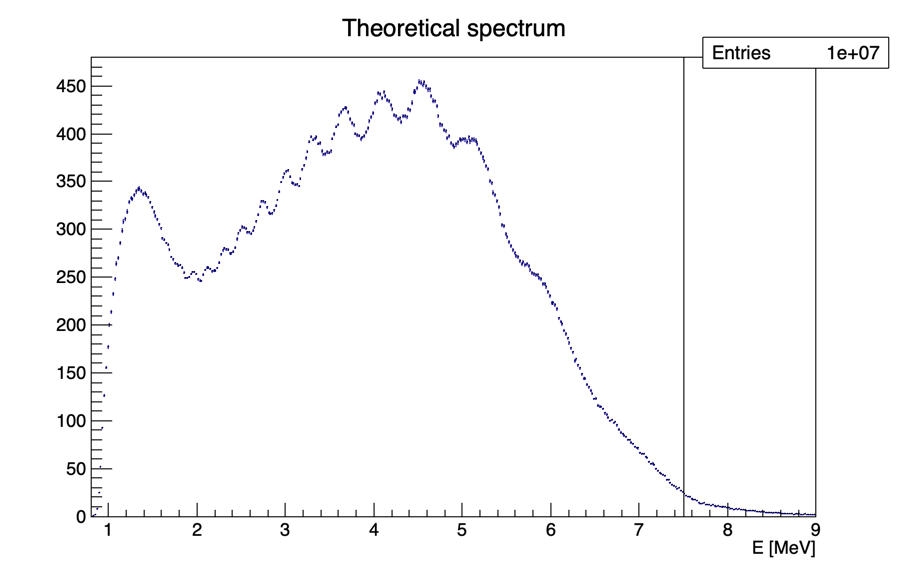
\includegraphics[height=6cm]{images/joint_fit/theoretical_spectrum.png}
  \caption{Theoretical LPMT spectrum at nominal oscillation values binned using 410 from 0.8 to 9 MeV. It is rescaled to correspond to the amount of event expected in 6 years of data taking. The black line represent the 335 bin cut}
  \label{fig:joint_fit:delta:theo}
\end{figure}

All the IBD spectra presented and used in this study are produced assuming Normal Ordering using the PDG nominal value \cite{particle_data_group_review_2020} for oscillation parameters. Those values are reported in table \ref{tab:joint_fit:pdg_value}.

%
%   (d) Les suppositions
%
%       --- Nous travaillons en traitant que des erreurs statistiques. Cela se justifie pour un travail exploratoire dans la mesure où une grande partie des effets syst sont totalement corrélés (ceux qui affectent le spectre vrai des neutrinos et des bruits de fond, voir table XX -- systèmatiques du papier Subpercent. )
%
%        --- L'essentiel de nos résultats supposent les effets de détection décorrélés entre LPMT et sPMT. Ils sont par ailleurs introduits de manière simpliste (simple tirage gaussien supposant une résolution gaussienne ne dépendant pas de la position de l'intéraction dans le détecteur --conforme à la publi Subpercent et à la dernière publi NMO). Ce choix se justifie pour un travail exploratoire par la nécessité de produire un grand nombre de toys malgré une puissance de calcul limitée. Un premier raffinement de cette approche tenant compte des corrélations entre les deux reconstructions est présenté en fin de chapitre. Il s'appuie sur la simulation complète du détecteur, et sur notre algo CNN de reco sPMT, le seul disponible à ce jour.
%
%        ---- La QNL est introduite de manière un peu simpliste pour l'instant (appliquée à nouveau juste en fonction de l'énergie de l'IBD). Rappeler que tu as tout de même établi une correspondance (alpha_qnl vs. gamma_qnl) en commençant à faire le boulot qu'il faudrait faire : l'appliquer au niveau des PMT (ce qui tient compte des effets de position de l'intéraction).

\subsection{Limitations}

In this work we are only working considering the statistical errors. We can ignore systematic effects, such as effects that would affect the neutrino spectrum or the background spectrum, as they are entirely correlated between the two systems. The details of those systematic effects can be found in \cite{juno_collaboration_sub-percent_2022}.

Most of our results assume decorrelated detection effects between the SPMT and LPMT system. Their respective reconstruction effect are simulated using simple gaussian drawing on the resolution, independent from their position. This approach was used in previous sensibility and precision studies \cite{juno_collaboration_sub-percent_2022, abusleme_potential_2024}. The potential effect of those reconstruction effects and a first attempt to take them into account are explored in section \ref{sec:joint_fit:cov_mat}.

Even if the goal of this work is to propose deformation agnostic tools, the QNL we use in this study is simplistic as we consider event-wise, position uniform deformation. We show in figure \ref{fig:joint_fit:ratio_distrib} and \ref{fig:joint_fit:gamma_v_alpha} that event-wise QNl is equivalent to the mean behaviour of channel-wise QNL but a more complete study would simulate channel-wise deformation for each event.

\section{Fit software}
\label{sec:joint_fit:framework}

In this section, I describe the ft framework that was used in this study. The software is composed of two part as illustrated in figure \ref{fig:joint_fit:framework}: A standalone part composed of ROOT \cite{brun_root-projectroot_2022} macros, and the Avenue framework.

The Avenue framework is responsible for the spectrum and configuration reading, transforming the raw collection of event into spectra, managing the physics effect such as the oscillation, computing and minimizing the $\chi^2$ with the help of the RooFit library. The macros are invoking, if necessary, the Avenue framework and are the entry point for fitting, generating the necessary inputs quantity such as the spectra and correlation matrix, analysing the fit results and managing jobs for distributed computing.

\begin{figure}[ht]
  \centering
  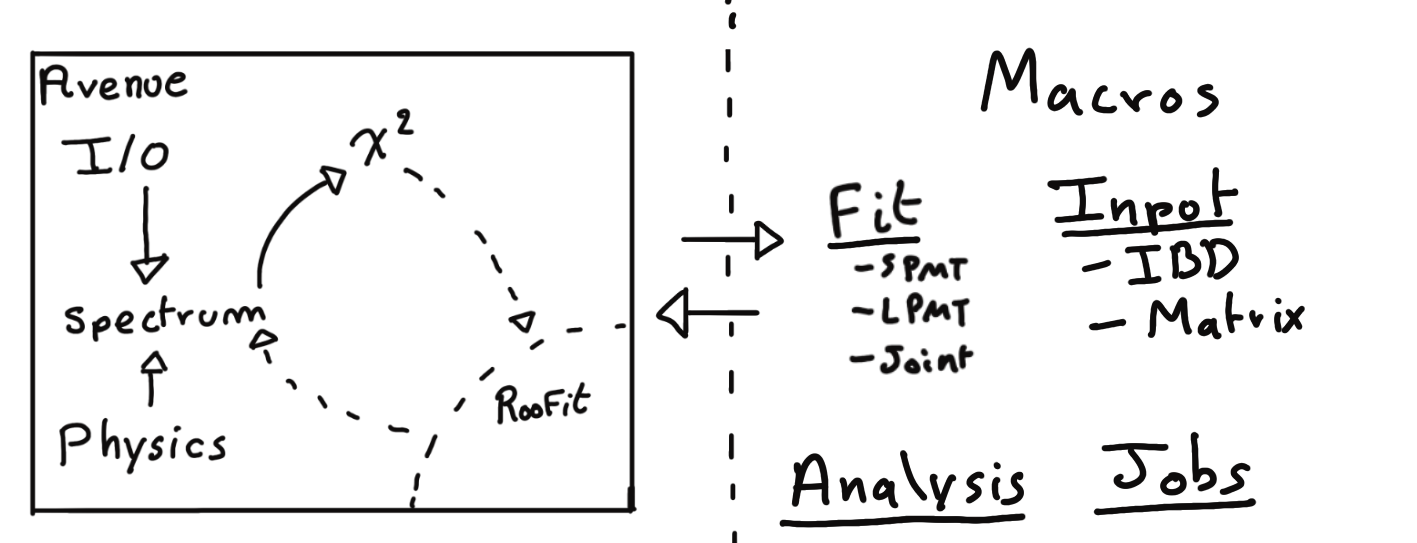
\includegraphics[height=6cm]{images/joint_fit/fit_framework.png}
  \caption{Schematic description of the fit framework}
  \label{fig:joint_fit:framework}
\end{figure}

In this section we will focus on the IBD generator in section \ref{sec:joint_fit:framework:ibd-gen} and the fit macro in itself in section \ref{sec:joint_fit:framework:fit}.
% IV) Le framework de fit.
% ---------------------------------------
%
% ... Description plus ou moins détaillée suivant qu'il a, ou non, déjà été décrit ailleurs...
%
%   (a) Introduction avec rapide overview
%
%
%   (b) La partie standalone : IBD-gen
\subsection{IBD generator}
\label{sec:joint_fit:framework:ibd-gen}

The IBD generator is a standalone generator used to produce oscillated and non oscillated spectrum as seen in the JUNO experiment. It takes as inputs physics parameters and a collection of histograms, values and function provided by JUNO to its analysis groups referred as the JUNO common inputs.

The arguments allow to enable or disable effect such as non-uniformity and non-linearity. It finally take as an argument the number of event to generate $N_{evt}$. Optionally, we generate an effective number of event $N$ by drawing in a Poisson distribution of mean $N_{evt}$.

Then for each event we
\begin{enumerate}
  \item Choose randomly following the reactor power fraction the reactor from which the neutrino come.
  \item Generate a random position in the detector following a uniform distribution in the detector.
  \item Draw a random neutrino energy $E_{\nu}$ from the expected neutrino emission spectrum of every reactor. This spectrum is calculated by:
    \begin{enumerate}
      \item Computing the power spectrum of each isotopes $^{235}$U, $^{238}$U, $^{239}$Pu, $^{241}$Pu using the Huber-Mueller model \cite{huber_determination_2011, mueller_improved_2011}.
      \item Summing the contribution of each isotopes following the respective fission fraction [0.58, 0.07, 0.30, 0.05] as reported in \cite{ma_improved_2013}.
      \item The power of each reactor is then adjusted by their distance from the detector, the detector efficiency and their mean duty cycle (11 of 12 month).
      \item The total spectrum is then finally adjusted by taking into account the correction of the Day Bay bump \cite{daya_bay_collaboration_measurement_2016}, adjustment due to spent nuclear fuel and due to the non-equilibrium.
    \end{enumerate}
  \item \textit{(Optional)} Compute the survival probability due to oscillation at nominal oscillation parameters value. If the neutrino does not survive, the event is rejected and start from step (1).
  \item Compute the emitted positron energy $E_{pos}$ from the mass difference. If the neutrino does not have enough energy reject the event and start from step (1).
  \item Compute the deposited energy $E_{dep}$ by incrementing $E_{pos}$ by 511 keV to account for the positron annihilation. We do not consider cases where some of the energy leak outside of the detector.
  \item Correct the deposited energy with the expected event-wise non-linearity from \cite{juno_collaboration_calibration_2021} to obtain the visible energy $E_{vis}$.
  \item \textit{(Optional)} Add a custom non-linearity as described in section \ref{sec:joint_fit:qnl}. This non linearity is characterized by $\alpha_{qnl}$ to obtain $E_{\alpha}$.
  \item Finally, using the expected resolution of the LPMT and SPMT system provided in the JUNO common inputs, we draw from a gaussian characterized by those resolution the reconstructed energy $E_{rec}$ or $E_{lpmt}$ and $E_{spmt}$ for each system.
\end{enumerate}

The events are stored as n-tuples and are not yet bin at the end of this step.

%
%   (c) Le framework de fit intégré.

\subsection{Fit}
\label{sec:joint_fit:framework:fit}

The fit macro is the core of this fitting procedure. This macro is responsible for loading the fit configuration and setup the Avenue framework. Using Avenue, it will setup the data files, theoretical spectrum, choose the binning, $\chi^2$, etc... It also have the possibility to generate toys on the fly based on the theoretical spectrum. Given this theoretical spectrum we can randomize the bin content either by:
\begin{enumerate}
  \item Drawing the bin content in a Poisson distribution with the bin content as parameter.
  \item Drawing the bin content in a Gaussian distribution with the bin content as mean and variance. The bin content is then rounded to the nearest integer.
  \item Drawing the bin difference following a given covariance matrix using the Choleski decomposition. This matrix is at least the statistical covariance matrix but can also contain systematic uncertainties.
    \begin{align}
      V &= LL^T \\
      \mathbf{R} &\sim \mathcal{N}(0, 1) \\
      \tilde{\mathbf{h}} &= \lceil \mathbf{h} + L\mathbf{R} \rfloor \\
    \end{align}
    where $V$ is covariance matrix used to produce the fluctuations, $\mathbf{R}$ is a draw in a multinomal distribution of mean 0 and variance 1, $\mathbf{h}$ the bin content of the theoretical spectrum and $\tilde{\mathbf{h}}$ the bin content of the generated toy.
\end{enumerate}

The first two methods allow for the fast production of statistics toys while the third allow for the production of statistical and systematical dependent toys. Unfortunately, none of those methods are fitted to produce toy with a QNL different from the theoretical spectrum. The uncertainty on the reconstructed energy $\sigma E_{rec}$ being dependent on $E_{vis}/E_{\alpha}$ makes that we would need to deconvolute the reconstruction effect from the theoretical spectrum. It is much easier to just produce those toys from the IBD generator.

% V) Tes développements techniques.
% -----------------------------------------------------------
%
%   (a) Pour générer les divers toys et pdf dont on a besoin, avec ou sans QNL.
%      --- Bien préciser les deux façons de générer des toys : dans IBDgen, ou dans le fmwk intégré, à partir de la matrice de corr et de Choleski.
%
%    (b)  Pour que le framework intégré soit capable de faire un fit joint.
%
% À ce stade, le lecteur doit comprendre comment tout est fait en pratique, et réaliser la quantité de travail technique que cela a demandé.
\section{Technical challenges and development}
\label{sec:joint_fit:tech}

The fit framework Avenue was already partially developed with multispectrum fitting in mind but a lot technical development was necessary to allow for a joint fit. The first step was to migrate the framework from ROOT5 (last release in March 2018) to ROOT6 (v6.26.06 released in July 2022) to ensure compatibility with the data coming from the JUNO collaboration and benefit of the improvement and corrections that came with ROOT6. This allow us to upgrade the C++ standard from C++11 to C++17. A substantial effort has been done to modernize the code, generalizing the function via templating to help readability and using smart pointer to prevent possible memory leaks.

The Avenue framework had to be adapted, notably on the chi-square calculation and spectrum generation to correctly take into account the correlation between the SPMT and LPMT spectrum. The delta joint fit requiring two more parameters over a spectrum twice as large as before with LPMT takes much more time, around 15h for 6 years exposure, than the single LPMT fit. Thus the framework and the fit macro had to be updated with ditributed calculation in mind. Notably the aggregation of fit results could be done in a single file instead of managing a file per fit. In case of numerous toy, the hard drive access time could lead to long analysis time.

While the IBD generator was already able to generate LPMT and SPMT spectrum, it was not designed for generating correlated spectrum. As detailed in section \ref{sec:joint_fit:framework:ibd-gen}, up to the reconstruction effect, the two spectrum need to share the same generation else the two spectrum would be decorelated and it would be like we would run two different experiment.

\section{Results}
\label{sec:joint_fit:results}
% VI) Résultats
% ----------------------
%
%    (a) Validations techniques.
%
%        i- Les test Asimov sans QNL que nous avions faits, pour valider que le fit joint est OK techniquement (joint vs. Moyenne pondérée des fit individuels) et notamment que la matrice a été mise correctement.
%
%        ii- Tous les autres que je n'ai plus en tête.

\subsection{Validation}

The first step is to confirm that the updated fit framework is able to reproduce existing results and that the joint fit behave as expected, meaning
\begin{itemize}
  \item Without QNL, the individual (\textit{LPMT} and \textit{SPMT}) fit converge to the parameter nominal value and that their errors in the ones reported in existing analysis such as \cite{juno_collaboration_sub-percent_2022}.
  \item The standard joint fit with an independent covariance matrix (\textit{Indep Standard joint}), meaning that the covariance between the LPMT and SPMT spectra is 0, believe to have twice as much information and thus believe to have a grater precision than the the individual fits.
  \item The standard joint (\textit{Standard joint}) fit but with a correlated covariance matrix has errors similiar to the LPMT individual fit as the LPMT drive the precision on $\theta_{13}$ and $\Delta m^2_{31}$ and that the LPMT as SPMT are expected to have the same precision on $\theta_{12}$ and $\Delta m^2_{21}$.
  \item The delta joint (\textit{Delta joint}) fit with covariance matrix have the same resolution as the standard joint fit. The supplementary parameter $\delta \theta_{12}$ and $\delta \Delta m^2_{21}$ should not bring supplementaty precision.
\end{itemize}

The italicized name are the name used in the results reports to identify each fit. We also look into the \textit{Indep Delta joint} which is the fit with the supplementary delta parameters but the covariance between the LPMT and SPMT spectra is 0 and the \textit{Weighted} results where
\begin{equation}
  \frac{1}{\sigma^2_{Weighted}} = \frac{1}{\sigma^2_{LPMT}} + \frac{1}{\sigma^2_{SPMT}}
\end{equation}
We expect the weighted resolution to be similar to the \textit{Indep Standard joint} as, in both of those test, we do not consider the correlation between the SPMT and LPMT results.

\subsubsection{Asimov studies}

We ran the the tests presented above on the updated framework, the results are reported in table \ref{tab:joint_fit:asimov_results}. All those test are ran considering statistics error only, 6 years exposure with all backgrounds, Pearson $\chi^2$ (covariance is estimated using data spectrum) and $\theta_{13}$ fixed to nominal value. For the \textit{SPMT} fit $\Delta m^2_{31}$ is fixed at nominal value as the SPMT system is net expected to be sensitive to this parameter.

\begin{table}[ht]
  \begin{footnotesize}
  \centering
  \begin{tabular}{l | c | c | c | c | c | c }
                                    & $\Delta m^2_{21}$ error  & $\delta \Delta m^2_{21}$ error & $\theta_{12}$ error   & $\delta \theta_{12}$ error  & $\Delta m^2_{31}$ error & $\chi^2$ \\
                                    \hline
  LPMT                                 & 1.29936e-07   &               & 1.33852e-03   &               & 4.39399e-06   & 3.23088e-18 \\
  SPMT                                 & 1.38297e-07   &               & 1.38653e-03   &               &               & 2.87502e-18 \\
  Indep Standard joint                 & 9.48731e-08   &               & 9.86765e-04   &               & 4.39212e-06   & 6.10592e-18 \\
  Standard joint                       & 1.29723e-07   &               & 1.18342e-03   &               & 4.39287e-06   & 3.38055e-18 \\
  Weighted                             & 9.46966e-08   &               & 9.63002e-04   &               &               & \\
  \hline
  Delta joint                            & 1.35780e-07   & 3.43529e-08   & 1.38236e-03   & 1.46865e-04   & 4.39309e-06   & 3.38055e-18 \\
  Indep Delta joint                      & 1.38297e-07   & 1.89391e-07   & 1.38653e-03   & 1.87830e-03   & 4.39241e-06   & 6.10592e-18 \\
  \hline
  \hline
  \multicolumn{7}{c}{Fixed $\Delta m^2_{21}$ and $\Delta m^2_{31}$} \\
  \hline
  Indep Standard joint &               &               & 9.33082e-04   &               &               & 4.82955e-26 \\
  LPMT                 &               &               & 1.27032e-03   &               &               & 2.58849e-26 \\
  SMPT                 &               &               & 1.31070e-03   &               &               & 2.24106e-26 \\
  Weighted             &               &               & 9.12193e-04   &               &               & \\
  \hline
  \hline
  \multicolumn{7}{c}{Fixed $\Delta m^2_{31}$ and$\theta_{12}$} \\
  \hline
  Indep Standard joint          & 8.97117e-08   &               &               &               &               & 6.10617e-18 \\
  SPMT                          & 1.30734e-07   &               &               &               &               & 2.87522e-18 \\
  LPMT                          & 1.23319e-07   &               &               &               &               & 3.23095e-18 \\
  Weighted                      & 8.97066e-08   &               &               &               &               & \\
  \end{tabular}
  \end{footnotesize}
  \caption{Results of the asimov studies of the updated framework. All results are asimov fit, considering 6 years exposure, $\theta_{13}$ is fixed to nominal value, $\chi^2$ is pearson meaning that he error is esitmated using the data spectrum}
  \label{tab:joint_fit:asimov_results}

\end{table}

In every cases presented above, the fit converges to the parameters nominal value thus only the errors are presented.

We observe, as expected, that $\sigma_{Weighted} \approx \sigma_{Indep~Standard~joint}$ with the exception of $\sigma \theta_{12}$. This could from the slight difference in statistic between the SPMT and LPMT spectra. Indeed, due to a larger smearing in energy resolution, event that would be in the spectra range [0.8, 7.5] MeV are smeared outside the spectrum. This deficit is partially compensated by event outside the spectrum coming back in this range but we expect very few event outside the spectrum in comparison to event at the edges of it. Thus the event deficit is not totally compensated. $\theta_{12}$ being mainly driven by the amplitude of the spectrum (see illustration \ref{fig:juno:juno-spectrum-oscillation}), that's why we think this the origin of the difference.

The second observation is that $\sigma_{Standard~joint} \approx \sigma_{LPMT}$. Once the covariance matrix between the LPMT and SPMT is correctly introduced, the fit ``understand'' that it does not have supplementary information and the LPMT system, which have the best precision, dominate the resolution.

Finally for the \textit{Delta} fit, the error on $\delta \theta_{12}$ and $\delta \Delta m^2_{21}$ are of the same order of magnitude than the errors on $\theta_{12}$ and $\Delta m^2_{21}$ in the absence of the covariance matrix. As the LPMT and SPMT spectra are not connected through the covariance matrix, the delta parameters are unconstrained thus the similar errors. Once the covariance matrix is introduced, the delta are much more constrained and present errors an order of magnitude smaller than the error om their respective parameters.

Overall, the asimov studies are satisfactory. The joint fit behave as expected and the errors on the delta parameters are significantly smaller than the error on their respective parameters, indicating great potential if the converge to value different from 0.

\subsubsection{Toy studies}

Once we validated that the asimov study is yielding coherent results, we study the behaviour of toy studies. The above asimov study is using the Pearson $\chi^2$ (Eq. \ref{eq:joint_fit:pearson}) without pull parameter, we show in figure \ref{fig:joint_fit:abs_standard_pearson} the effect of using a simple Pearson $\chi^2$. We see that $\sin^2(2\theta_{12})$ (reported as $\theta_{12}$ for simplicity) is biased of about $0.5\sigma$ and $\Delta m^2_{21}$ biased of about $0.1\sigma$. When introducing the PearsonV $\chi^2$ (Eq. \ref{eq:joint_fit:pearsonV}) the bias disappear as reported in figure \ref{fig:joint_fit:abs_standard_pearsonV}.

\begin{figure}[ht]
  \centering
  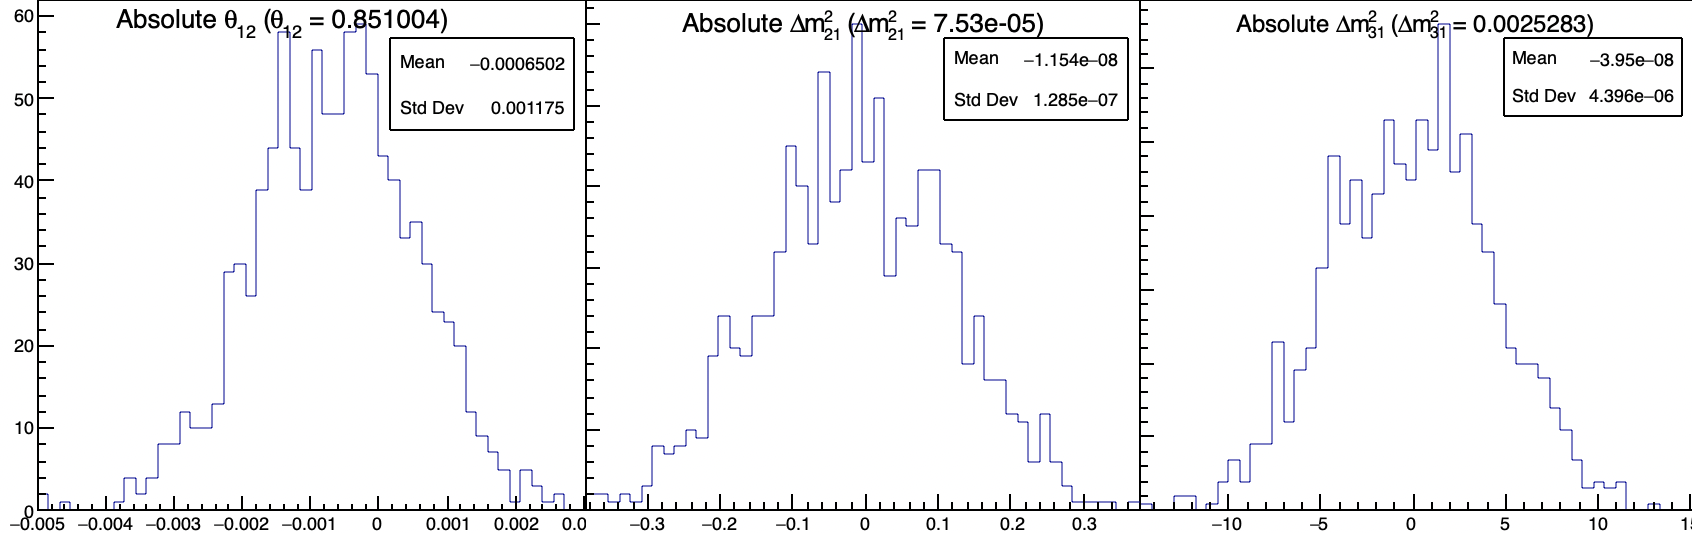
\includegraphics[width=\linewidth]{images/joint_fit/absolute_standard_joint_pearson.png}
  \caption{Distribution of BFP - nominal value for 1000 toy Standard joint fit. 6 years exposure, all background, \textbf{Pearson} $\chi^2$, $\theta_{13}$ fixed.}
  \label{fig:joint_fit:abs_standard_pearson}
\end{figure}

\begin{figure}[ht]
  \centering
  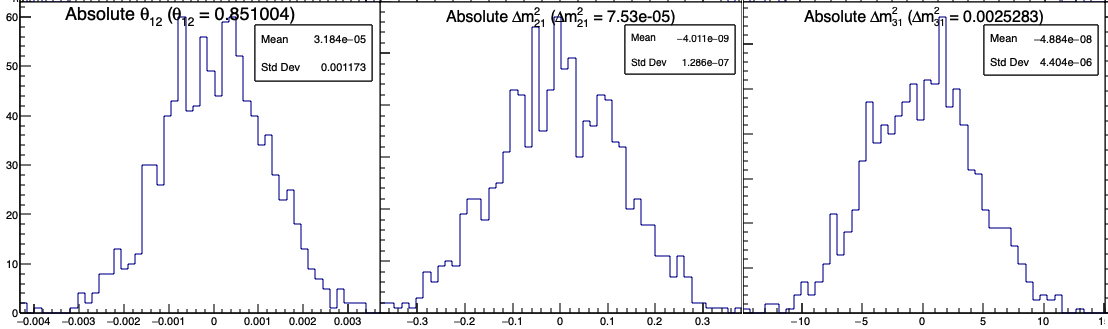
\includegraphics[width=\linewidth]{images/joint_fit/absolute_standard_joint_pearsonV.png}
  \caption{Distribution of BFP - nominal value for 1000 toy Standard joint fit. 6 years exposure, all background, \textbf{PearsonV} $\chi^2$, $\theta_{13}$ fixed.}
  \label{fig:joint_fit:abs_standard_pearsonV}
\end{figure}

When the supplementary parameters are introduced in the Delta Joint fit, the fit is stable as shown in the results figure \ref{fig:joint_fit:delta_fit}. The resolutions on the oscillation parameters are slightly worse in the Delta joint fit due to the supplementary freedom. As seen in the asimov studies, the resolution of the $\delta$ parameters is an order of magnitude smaller than their respective parameters, indicating that they can be powerful tools to detect discrepancies between the SPMT and LPMT spectra.

\begin{figure}[ht]
  \centering
  \begin{subfigure}[t]{0.98\linewidth}
    \centering
    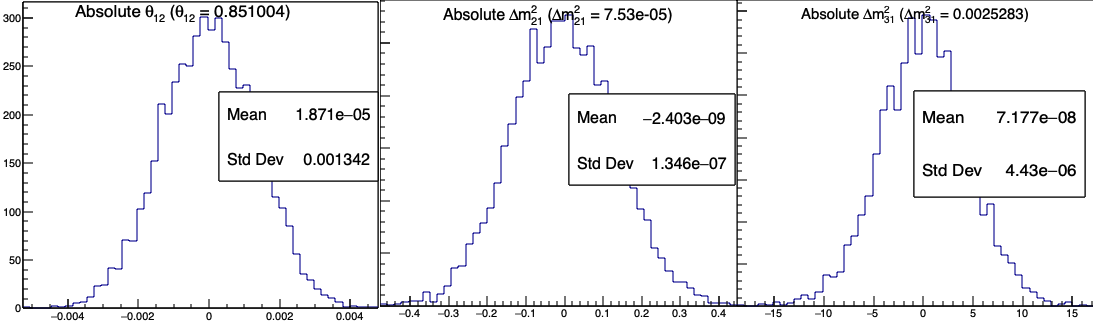
\includegraphics[width=\linewidth]{images/joint_fit/normal_delta_joint.png}
  \end{subfigure}

  \begin{subfigure}[t]{0.66\linewidth}
    \centering
    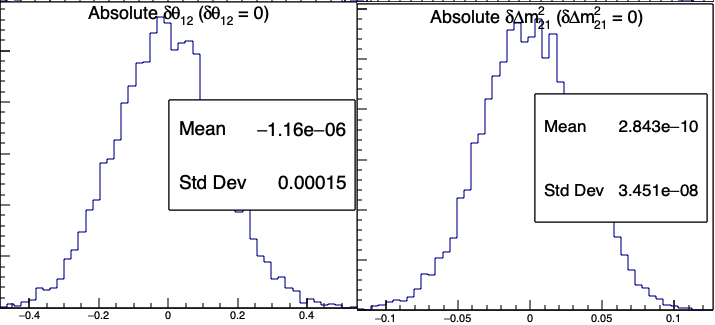
\includegraphics[width=\linewidth]{images/joint_fit/supp_delta_joint.png}
  \end{subfigure}

  \caption{Distribution of BFP - nominal value for 5000 toy Delta joint fit. 6 years exposure, all background, \textbf{PearsonV} $\chi^2$, $\theta_{13}$ fixed.}
  \label{fig:joint_fit:delta_fit}
\end{figure}

\subsubsection{Effect of supplementary QNL on the LPMT spectrum}

Now that we know that the framework and joint fit behave correctly on unbiased data, we test the effect of introducing the QNL, as presented in Eq. \ref{eq:joint_fit:alpha_yang}, in the LPMT spectrum. To test the effect, we consider a QNL $\alpha_{qnl} = 1\%$. For reference, this is about three time the expected residual QNL after calibration ($\alpha_{qnl} = 0.3\%$ \cite{juno_collaboration_calibration_2021}). We use a covariance matrix assuming no QNL. The effect of this QNL on the spectrum is illustrated in figure \ref{fig:joint_fit:anom_aqnl}. In table \ref{tab:joint_fit:qnl_results} we report the results of the different scenarios.

\begin{figure}[ht]
  \centering
  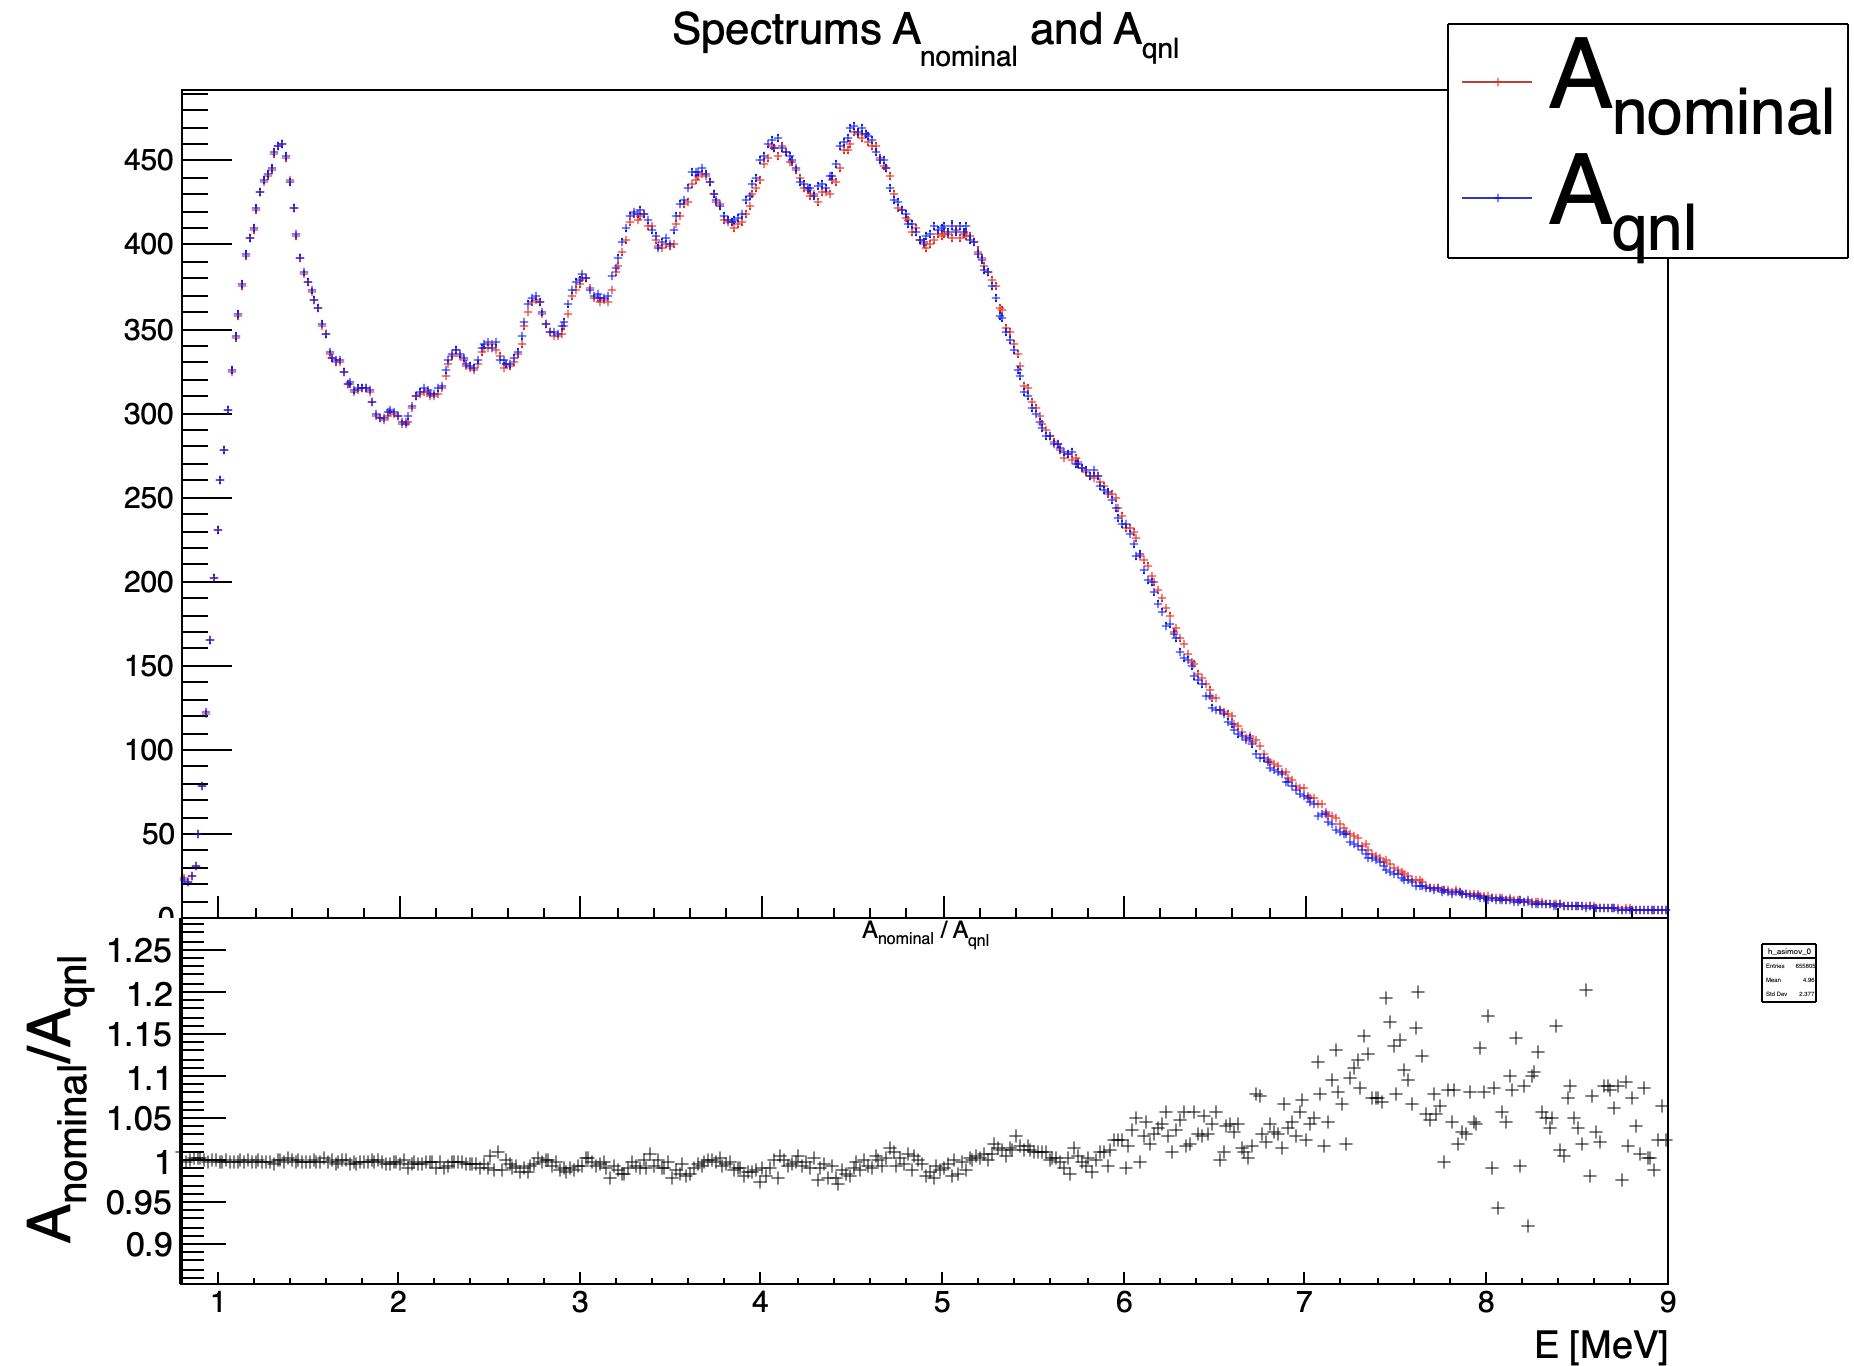
\includegraphics[height=6cm]{images/joint_fit/AnominalAQNL.png}
  \caption{\textbf{Top:} Theoretical spectrum without QNL (in red) and with $\alpha_{qnl} = 1\%$ (in blue). \textbf{Bottom:} Ratio between the theoretical spectrum with and without QNL.}
  \label{fig:joint_fit:anom_aqnl}
\end{figure}



%\begin{table}
%  \begin{footnotesize}
%  \centering
%  \begin{tabular}{l|lr|lr|lr|lr|lr|}
%    Mean (standard deviation)  & \multicolumn{2}{c|}{$\theta_{12}$} & \multicolumn{2}{c|}{$\Delta m^2_{21}$} & \multicolumn{2}{c|}{$\Delta m^2_{31}$} & \multicolumn{2}{c|}{$\delta \theta_{12}$} & \multicolumn{2}{c|}{$\delta \Delta m^2_{21}$} \\
%    \hline
%    LPMT            & -0.904 & (0.968) & -0.3141 & (0.998)   &  -1.74         & (0.992)           &\multicolumn{2}{c|}{Irrelevant} & \multicolumn{2}{c|}{Irrelevant}  \\
%    SPMT            & 0.188  & (0.975) & -0.0752 & (1.019)   & \multicolumn{2}{c|}{Not sensitive} &\multicolumn{2}{c|}{Irrelevant} & \multicolumn{2}{c|}{Irrelevant}  \\
%    Indep Standard  & -0.502 & (1.328) & -0.2758 & (1.407)   & -1.731         & (0.992)           &\multicolumn{2}{c|}{Irrelevant} & \multicolumn{2}{c|}{Irrelevant}  \\
%    Standard        & -6.01  & (1.201) & -1.511  & (1.031)   & -1.82          & (1.275)           &\multicolumn{2}{c|}{Irrelevant} & \multicolumn{2}{c|}{Irrelevant}  \\
%    Indep Delta     & 0.184  & (0.973) & -0.704  & (1.019)   & -1.737         & (0.990)           & -0.787     & (0.146) & -0.168 & (0.219) \\
%    Delta           & 0.136  & (0.974) & -0.687  & (1.028)   & -1.74          & (0.993)           & -10.88     & (1.628) & 1.727  & (0.995)
%  \end{tabular}
%  \end{footnotesize}
%  \caption{Results of the different fit scenarios on QNL distorted data $\alpha_{qnl} = 1\%$. For SPMT $\Delta m^2_{31}$ is fixed at nominal value. The $\chi^2$ is PearsonV. The correlation matrix used to fit suppose no QNL in the spectrum.}
%  \label{tab:joint_fit:qnl_results}
%\end{table}




%   (b) La matrice de covariance
%
%      i- méthode théorique
%         --- explications
%         --- résultats
%      ii- méthode toys
%             Idem
%      iii- la méthode basée sur les données sniper.
%            Idem
%      iv- comparaison
%         --- commentaires et conclusion.
%
%     Préciser ou rappeler ici que
%         --- pour nos tests, nous nous basons sur l'hypo H0 et donc nous générons la matrice sans QNL.
%         --- les corrélations dépendent peu de la forme du spectre ou se sa stat.
\subsection{Covariance matrix}
\label{sec:joint_fit:cov_mat}

%
%   (c) Résultats fit séparés
%
%
%   (d) Résultats fits joints
%
%   (e) Résultats avec corrélations reco_spmt vs. reco_lmpt mieux prises en compte
%

\section{Conclusion and perspectives}
\label{sec:joint_fit:conclusion}
% Vll) Discussions, perspectives

\end{document}
